\scanpage{61}
Groupes finis sur base de car. $p>0$.

\uline{Groupes finis étales}

Soit $G$ fini étale annulé par $p^n$. Pour tout épaississement
$S'$ de $S$, $G$ s'étend de façon unique en un groupe fini étale
$G'$ sur $S'$, également tué par $p^n$. Soit
$\mathcal M_{S'}=G'\otimes_{\mathbb Z/p^n\mathbb Z}
\underline{\mathcal O}_{S'}
=G'\otimes_{\mathbb Z/p^n\mathbb Z}
(\mathcal O_{S'}/p^n\mathcal O_{S'})$.
Pour $S'$ variable, on obtient un cristal $\mathbb D_*(G)$.
L'hom $G\xrightarrow{f}G^p$ est ici un isom. et définit un hom
\[
\unsure{F_*|F_\bullet}:\mathbb D_*(G)-\mathbb D_*(G)^{(p)}
\]
qui est un isomorphisme. Par dualité, posant
\[
\check G=\underline{\operatorname{Hom}}_{\mathrm{gr}}
(G,(\mathbb Q_p/\mathbb Z_p)_S),\qquad
\mathbb D^*(G)=\mathbb D_*(\check G)
\]
on trouve un \inserted{anti-}foncteur $G\longmapsto\mathbb D^*(G)$,
et
\[
F^*:\mathbb D^*(G)^{(p)}\xrightarrow{\sim}\mathbb D^*(G).
\]
$V^*$ est uniquement défini par $\deleted{\mathbb D^*(G)}$.
$F^*V^*=p\operatorname{id}_{\mathbb D^*(G)}$.

\deleted{\unsure{On} Dans la catégorie des cristaux de modules}

\uline{Cas}\quad $G$ \uline{plat sur} $\Lambda_n$
(i.e. groupe à B.T. tronqué d'échelon $n$).
Alors $\mathbb D^*(G)$ est un cristal de modules loc. libre de t.f.
rel. à $\Lambda_n$, \unsure{\&} avec $F$ \deleted{tel que}
un isomorphisme ($\mapsto V$ de façon unique) et on obtient une
\inserted{anti-}équivalence de la catégorie des
\deleted{\unsure{cris}} $G$ et des $F$-cristaux précédents.
\margin{\uline{vérifier}}
\figure{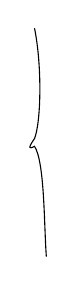
\begin{tikzpicture}
\draw (0,1.5) .. controls (.1,1) and (.08,.3) .. (0,.1)
.. controls (-.08,-.02) and (-.08,-.04) .. (0,0)
.. controls (.13,-.2) and (.12,-1) .. (.15,-1.4);
\end{tikzpicture}}

\uline{Cas général}\quad \inserted{Anti-}Équivalence entre la catégorie
des $G$, et celle des \inserted{$F$-}cristaux
(i.e. $F$-$V$-cristaux) sur $S$ qui loc. (ét) sont des sommes de
cristaux du type précédent (avec $n$ variable).

De ceci résulte que si $G\longleftrightarrow M$, on a
\[
G(S)\underset{\unsure{n\ \mathrm{grd.}}}{\simeq}
\operatorname{Hom}_{\mathrm{gr}}(\Lambda_{nS},G)
\simeq\operatorname{Hom}_{F-V-\mathrm{cris}}
(M,\mathcal O_{S,n\,\mathrm{cris}})
\simeq\operatorname{Hom}_{F-\mathrm{cris}}(\unsure{-})
\]
\margin{71}
